\documentclass{beamer}
\usetheme{Darmstadt}
\usecolortheme{whale}
\usepackage[utf8]{inputenc}
\usepackage{lmodern}


%\titlegraphic{
\includegraphics[width=2cm]{images/uadec-logo}\hspace*{4.75cm}~%
%   
\includegraphics[width=2cm]{images/uadec-logo}
%}
\logo{

\includegraphics[height=1cm]{images/uadec-logo}
\hspace{\dimexpr\textwidth-3.5mm} 
\includegraphics[height=0.75cm]{images/uadec-logo-2}
}
\title{My research plan for the master's program}
\author{Suresh Kumar Gadi}
\date{20$^{\mbox{th}}$ December 2016}
\institute{FIME-UT, UAdeC}
\begin{document}

\frame{\titlepage}
\begin{frame}{Overview}
	\tableofcontents
\end{frame}
\section{Independent research}
\subsection{Some of the emerging research topics}
\begin{frame}{Examples of independent research topics}
	\begin{itemize}
		\item Maximum Power Point Tracking (MPPT)
		\item Hybrid power supplies
	\end{itemize}
\end{frame}
\subsubsection{Maximum Power Point Tracking (MPPT)}
\begin{frame}[allowframebreaks]{Maximum Power Point Tracking (MPPT)}
	\begin{block}{Problem statement}
		Renewable energies are not constant power suppliers. MPPT is a controller, usually an electronic circuit implementing an algorithm to extract the maximum possible power from the renewable energy source at all the times.
	\end{block}
	\framebreak
	\begin{center}
		\textbf{Defining MPPT}\\
		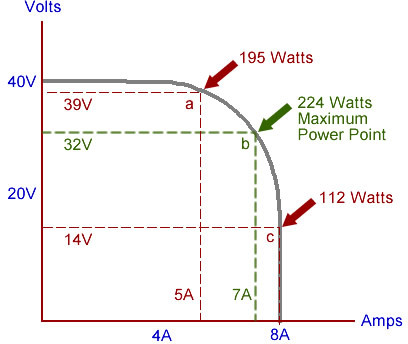
\includegraphics[height=6cm]{images/mppt-power-source}\\
		VI (Voltage-current) curve of a battery.
	\end{center}
	\framebreak
	\begin{center}
		\textbf{MPPT application to the photovoltaic (PV) cells}\\
		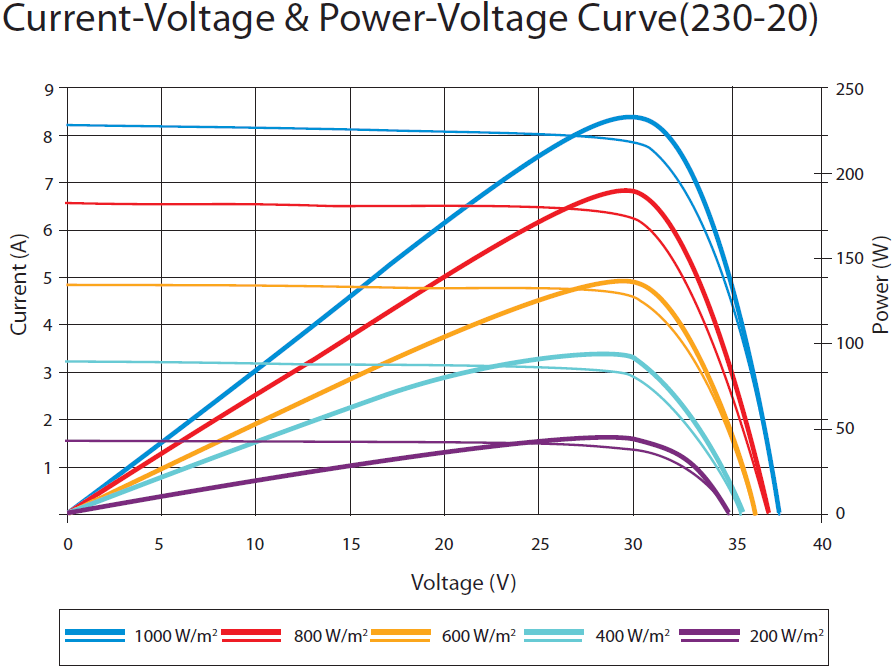
\includegraphics[height=6cm]{images/mppt-solar}\\
		PV current vs voltage curve at the various solar intensity.
	\end{center}
	\framebreak
	\begin{center}
		\textbf{MPPT application to wind mills}\\
		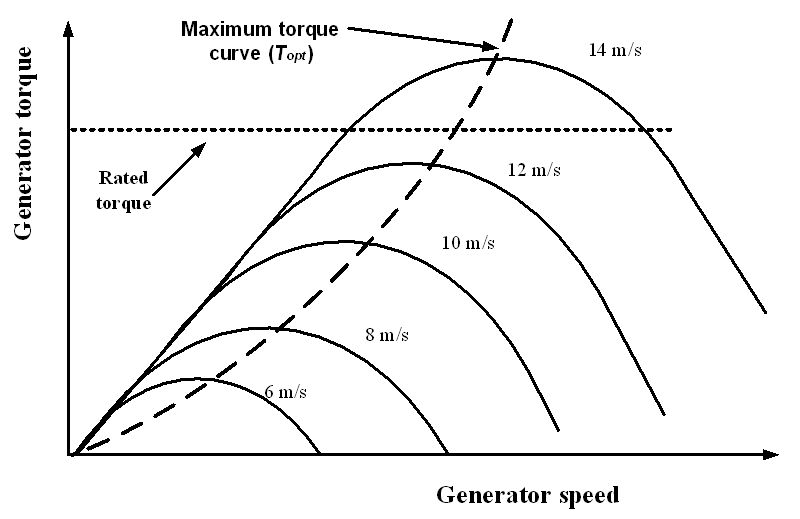
\includegraphics[height=6cm]{images/mppt-wind}\\
		Generator speed vs torque curve at the various wind speeds.% \cite{fox2007wind, eltamaly2013maximum}.
	\end{center}
	\framebreak
\end{frame}
\subsubsection{Hybrid renewable energy systems (HRES)}
\begin{frame}[allowframebreaks]{Hybrid renewable energy systems (HRES)}
	\begin{block}{Problem statement}
		\begin{itemize}
			\item Providing the solutions to grid independent renewable energy sources.
			\item Selection of capacity of each power source.
			\item Optimized switching between different power sources.
		\end{itemize}
	\end{block}
	\framebreak
\end{frame}
\subsection{Recommended student profile for the admission}
\begin{frame}{Recommended student profile for the admission}
\begin{itemize}
	\item Sciences: Basics of differential equations, basic classical physics
	\item Technology: Basic analog and digital electronics, control systems
	\item Computer knowledge: At least one programming language
\end{itemize}
\end{frame}
\subsection{Compulsory courses required for the master program}
\begin{frame}{Compulsory courses required for the master program}
	\begin{itemize}
		\item Courses: Advanced engineering mathematics, linear systems, linear algebra, mathematical modeling,
		\item Seminars: MatLab, real-time systems
	\end{itemize}
\end{frame}
\subsection{Optional courses required for the master program}
\begin{frame}{Compulsory courses required for the master program}
	\begin{itemize}
		\item Courses: Nonlinear systems, stochastic systems, adaptive control
		\item Seminars: C/C++, Python
	\end{itemize}
\end{frame}
\subsection{Target journals}
\begin{frame}{Target journals}
	\begin{tabular}{|p{7cm}|c|c|}
		\hline
		\textbf{Journal} & \textbf{I.P.} & \textbf{Review time} \\ \hline
		Renewable and Sustainable Energy Reviews & 7 & 1-2 years \\ \hline
		IEEE Transaction on Industry Application & 1.9 &  $>$1  \\ \hline
		Applied Energy & 5 & $\approx$ 1 \\ \hline
		Solar Energy & 3.7 & $>$1 \\ \hline
	\end{tabular}
\end{frame}
\section{Research support}
\subsection{Examples}
\begin{frame}{Examples of research support}
	\begin{itemize}
		\item Automation of a process
		\item Statistical and numerical analysis
	\end{itemize}
\end{frame}
\subsubsection{Automation of a process}
\begin{frame}{Automation of a process}
	\begin{block}{Examples}
		\begin{itemize}
			\item Building a custom signal conditioner circuit.
			\item Process control, i.e. Controlling flow, temperature etc. with high precision.
			\item Custom experimental setup.
		\end{itemize}
	\end{block}
	\framebreak
\end{frame}
\subsubsection{Statistical and numerical analysis}
\begin{frame}{Statistical and numerical analysis}
	\begin{block}{Examples}
		\begin{itemize}
			\item Organizing, making a computer program for collecting and processing data.
			\item Working in parallel to the experimenting professor to provide help with the mathematical part of the article to speed up publications.
		\end{itemize}
	\end{block}
	\framebreak
\end{frame}
\subsection{Recommended student profile for the admission}
\begin{frame}{Recommended student profile for the admission}
	\begin{itemize}
		\item Sciences: Basics of differential equations, basic classical physics
		\item Technology: Basic analog and digital electronics, control systems
		\item Computer knowledge: At least one programming language
	\end{itemize}
\end{frame}
\subsection{Compulsory courses required for the master program}
\begin{frame}{Compulsory courses required for the master program}
	\begin{itemize}
		\item Courses: Advanced engineering mathematics, linear systems, linear algebra, mathematical modeling,
		\item Seminars: MatLab, real-time systems
	\end{itemize}
\end{frame}
\subsection{Optional courses required for the master program}
\begin{frame}{Compulsory courses required for the master program}
	\begin{itemize}
		\item Courses: Nonlinear systems, stochastic systems, adaptive control
		\item Seminars: C/C++, Python
	\end{itemize}
\end{frame}
\appendix
\begin{frame}{}
	\centering {\huge{Questions?\\[2cm]Thank you for your attention.}}
\end{frame}

\end{document}
